\section{Results}
\label{sec:results}

\subsection{Main Performance}

Table~\ref{tab:main} compares PCGT against 13 baselines on 7 medium-scale datasets. Baseline results for GCN through SGFormer are taken from \citet{wu2023sgformer}; DIFFormer from \citet{wu2023difformer}; NAGphormer from \citet{chen2023nagphormer}; GraphGPS from our own runs using the Performer-attention implementation of \citet{rampasek2022graphgps}. PCGT numbers are from our own runs on an NVIDIA H100 GPU (10 runs each).

\begin{table*}[t]
\centering
\small
\setlength{\tabcolsep}{3pt}
\resizebox{\textwidth}{!}{%
\begin{tabular}{l|ccc|cccc}
\toprule
 & \multicolumn{3}{c|}{\textbf{Homophilic}} & \multicolumn{4}{c}{\textbf{Heterophilic}} \\
\textbf{Method} & \textbf{Cora} & \textbf{CiteSeer} & \textbf{PubMed} & \textbf{Film} & \textbf{Squirrel} & \textbf{Chameleon} & \textbf{Deezer} \\
\midrule
\multicolumn{8}{l}{\textit{Standard GNNs}} \\
GCN & 81.6{\scriptsize$\pm$0.4} & 71.6{\scriptsize$\pm$0.4} & 78.8{\scriptsize$\pm$0.6} & 30.1{\scriptsize$\pm$0.2} & 38.6{\scriptsize$\pm$1.8} & 41.3{\scriptsize$\pm$3.0} & 62.7{\scriptsize$\pm$0.7} \\
GAT & 83.0{\scriptsize$\pm$0.7} & 72.1{\scriptsize$\pm$1.1} & 79.0{\scriptsize$\pm$0.4} & 29.8{\scriptsize$\pm$0.6} & 35.6{\scriptsize$\pm$2.1} & 39.2{\scriptsize$\pm$3.1} & 61.7{\scriptsize$\pm$0.8} \\
APPNP & 83.3{\scriptsize$\pm$0.5} & 71.8{\scriptsize$\pm$0.5} & 80.1{\scriptsize$\pm$0.2} & 31.3{\scriptsize$\pm$1.5} & 35.3{\scriptsize$\pm$1.9} & 38.4{\scriptsize$\pm$3.5} & 66.1{\scriptsize$\pm$0.6} \\
SIGN & 82.1{\scriptsize$\pm$0.3} & 72.4{\scriptsize$\pm$0.8} & 79.5{\scriptsize$\pm$0.5} & 36.5{\scriptsize$\pm$1.0} & 40.7{\scriptsize$\pm$2.5} & 41.7{\scriptsize$\pm$2.2} & 66.3{\scriptsize$\pm$0.3} \\
\midrule
\multicolumn{8}{l}{\textit{Heterophily-Specific GNNs}} \\
H$_2$GCN & 82.5{\scriptsize$\pm$0.8} & 71.4{\scriptsize$\pm$0.7} & 79.4{\scriptsize$\pm$0.4} & 34.4{\scriptsize$\pm$1.7} & 35.1{\scriptsize$\pm$1.2} & 38.1{\scriptsize$\pm$4.0} & 66.2{\scriptsize$\pm$0.8} \\
CPGNN & 80.8{\scriptsize$\pm$0.4} & 71.6{\scriptsize$\pm$0.4} & 78.5{\scriptsize$\pm$0.7} & 34.5{\scriptsize$\pm$0.7} & 38.9{\scriptsize$\pm$1.2} & 40.8{\scriptsize$\pm$2.0} & 65.8{\scriptsize$\pm$0.3} \\
GloGNN & 81.9{\scriptsize$\pm$0.4} & 72.1{\scriptsize$\pm$0.6} & 78.9{\scriptsize$\pm$0.4} & 36.4{\scriptsize$\pm$1.6} & 35.7{\scriptsize$\pm$1.3} & 40.2{\scriptsize$\pm$3.9} & 65.8{\scriptsize$\pm$0.8} \\
\midrule
\multicolumn{8}{l}{\textit{Graph Transformers}} \\
NodeFormer & 82.2{\scriptsize$\pm$0.9} & 72.5{\scriptsize$\pm$1.1} & 79.9{\scriptsize$\pm$1.0} & 36.9{\scriptsize$\pm$1.0} & 38.5{\scriptsize$\pm$1.5} & 34.7{\scriptsize$\pm$4.1} & 66.4{\scriptsize$\pm$0.7} \\
DIFFormer & 83.5{\scriptsize$\pm$0.6} & 72.2{\scriptsize$\pm$0.5} & 79.7{\scriptsize$\pm$0.6} & 37.5{\scriptsize$\pm$1.0} & 39.5{\scriptsize$\pm$2.1} & 44.0{\scriptsize$\pm$3.5} & 66.4{\scriptsize$\pm$0.9} \\
NAGphormer & 83.2{\scriptsize$\pm$0.8} & 72.3{\scriptsize$\pm$0.4} & 78.6{\scriptsize$\pm$0.3} & 35.8{\scriptsize$\pm$1.1} & 38.3{\scriptsize$\pm$1.9} & 42.3{\scriptsize$\pm$3.1} & 66.7{\scriptsize$\pm$0.7} \\
GraphGPS & 78.6{\scriptsize$\pm$1.7} & 60.4{\scriptsize$\pm$1.4} & 75.5{\scriptsize$\pm$0.7} & 34.0{\scriptsize$\pm$0.6} & 36.5{\scriptsize$\pm$2.5} & 44.2{\scriptsize$\pm$3.5} & 67.0{\scriptsize$\pm$0.7} \\
SGFormer & \best{84.5}{\scriptsize$\pm$0.8} & \runup{72.6}{\scriptsize$\pm$0.2} & \runup{80.3}{\scriptsize$\pm$0.6} & \runup{37.9}{\scriptsize$\pm$1.1} & \runup{41.8}{\scriptsize$\pm$2.2} & \runup{44.9}{\scriptsize$\pm$3.9} & \runup{67.1}{\scriptsize$\pm$1.1} \\
\midrule
\textbf{PCGT (ours)} & \runup{84.3}{\scriptsize$\pm$0.4} & \best{73.1}{\scriptsize$\pm$0.4} & \best{81.0}{\scriptsize$\pm$0.6} & \best{38.0}{\scriptsize$\pm$0.9} & \best{45.5}{\scriptsize$\pm$2.7} & \best{49.0}{\scriptsize$\pm$2.8} & \best{67.2}{\scriptsize$\pm$0.7} \\
\bottomrule
\end{tabular}
}% end resizebox
\caption{Node classification accuracy (\%) on medium-scale benchmarks. Mean $\pm$ std over 10 runs (Deezer: 5 runs). GCN--SGFormer from \citet{wu2023sgformer}; DIFFormer from \citet{wu2023difformer}; NAGphormer from \citet{chen2023nagphormer}; GraphGPS from our runs. \best{Best} and \runup{runner-up} per column.}
\label{tab:main}
\end{table*}

Table~\ref{tab:new_datasets} reports results on four additional datasets where we run both SGFormer and PCGT under identical settings (10 runs each, random 50/25/25 splits).

\begin{table}[t]
\centering
\small
\setlength{\tabcolsep}{3pt}
\resizebox{\columnwidth}{!}{%
\begin{tabular}{l|cccc}
\toprule
\textbf{Method} & \textbf{Co-CS} & \textbf{Co-Phys} & \textbf{Am-Comp} & \textbf{Am-Photo} \\
\midrule
GCN & 91.9{\scriptsize$\pm$0.4} & 95.7{\scriptsize$\pm$0.2} & 82.8{\scriptsize$\pm$1.8} & 90.9{\scriptsize$\pm$1.2} \\
GAT & 92.0{\scriptsize$\pm$0.3} & 95.4{\scriptsize$\pm$0.2} & 83.4{\scriptsize$\pm$0.9} & 91.1{\scriptsize$\pm$0.8} \\
SGFormer & \runup{94.9}{\scriptsize$\pm$0.5} & \runup{96.6}{\scriptsize$\pm$0.2} & \runup{87.5}{\scriptsize$\pm$2.0} & \runup{95.2}{\scriptsize$\pm$1.2} \\
\textbf{PCGT (ours)} & \best{95.1}{\scriptsize$\pm$0.3} & \best{96.8}{\scriptsize$\pm$0.2} & \best{88.8}{\scriptsize$\pm$0.7} & \best{95.3}{\scriptsize$\pm$0.4} \\
\bottomrule
\end{tabular}}%
\caption{Accuracy (\%) on four additional datasets. Mean $\pm$ std over 10 runs. GCN and GAT baselines from our own runs on H100. \best{Best} and \runup{runner-up} per column.}
\label{tab:new_datasets}
\end{table}

\textbf{Heterophilic datasets.} The largest gains are on heterophilic benchmarks: +4.1\% on Chameleon and +3.7\% on Squirrel over SGFormer, which was already the previous best. PCGT beats all 13 baselines on these datasets, including heterophily-specific methods like GloGNN (+8.8\% on Chameleon) and H$_2$GCN (+10.4\% on Squirrel). On Film, PCGT also leads (38.0 vs.\ 37.9 for SGFormer).

\textbf{Homophilic datasets.} On CiteSeer, PCGT scores 73.1 vs.\ SGFormer's 72.6 (+0.5\%). On PubMed, 81.0 vs.\ 80.3 (+0.7\%). On Cora, the two are within noise (84.3 vs.\ 84.5). PCGT also shows lower run-to-run variance than SGFormer across these benchmarks.

\textbf{Additional datasets (Table~\ref{tab:new_datasets}).} PCGT wins on all four, outperforming not only SGFormer but also GCN and GAT baselines by large margins. Coauthor-Physics (+0.2\% over SGFormer) is statistically significant ($p$=0.004). Amazon-Computers has the largest absolute gap (+1.3\%, $p$=0.051). PCGT's variance is also consistently lower (e.g., $\pm$0.7 vs.\ $\pm$2.0 on Amazon-Computers).

\textbf{Mixed homophily (Deezer).} PCGT scores 67.2 vs.\ SGFormer's 67.1 on Deezer ($h \approx 0.5$), a +0.1\% gap that is within the error bars and not statistically significant. With a lower graph weight ($\lambda_{\text{gw}}=0.5$), PCGT gives more influence to the partition-conditioned attention, but the gain on this mixed-homophily dataset is marginal.

\subsection{Large-Scale Results}

To test scalability beyond medium-sized graphs, we evaluate on three large-scale benchmarks spanning homophilic and heterophilic regimes: ogbn-arxiv (169K nodes, 1.2M edges)~\citep{hu2020ogb}, pokec (1.6M nodes, 30.6M edges)~\citep{lim2021large}, and Amazon2M (2.4M nodes, 61.9M edges)~\citep{wu2022nodeformer}. We follow the mini-batch training setup of SGFormer~\citep{wu2023sgformer}. Baselines are from \citet{wu2023sgformer} Table~3.

\begin{table}[t]
\centering
\small
\resizebox{\columnwidth}{!}{%
\begin{tabular}{l|ccc}
\toprule
\textbf{Method} & \textbf{ogbn-arxiv} & \textbf{pokec} & \textbf{Amazon2M} \\
\midrule
MLP & 55.50{\scriptsize$\pm$0.23} & 60.15{\scriptsize$\pm$0.03} & 63.46{\scriptsize$\pm$0.10} \\
GCN~\citep{kipf2017semi} & 71.74{\scriptsize$\pm$0.29} & 62.31{\scriptsize$\pm$1.13} & 83.90{\scriptsize$\pm$0.10} \\
SIGN~\citep{rossi2020sign} & 71.95{\scriptsize$\pm$0.11} & 68.01{\scriptsize$\pm$0.25} & 80.98{\scriptsize$\pm$0.31} \\
NodeFormer~\citep{wu2022nodeformer} & 59.90{\scriptsize$\pm$0.42} & 70.32{\scriptsize$\pm$0.45} & 87.85{\scriptsize$\pm$0.24} \\
SGFormer~\citep{wu2023sgformer} & \best{72.63}{\scriptsize$\pm$0.13} & 73.76{\scriptsize$\pm$0.24} & \best{89.09}{\scriptsize$\pm$0.10} \\
\midrule
\textbf{PCGT (ours)} & \runup{72.50}{\scriptsize$\pm$0.14} & \best{74.94}{\scriptsize$\pm$0.28} & \runup{88.79}{\scriptsize$\pm$0.06} \\
\bottomrule
\end{tabular}
}% end resizebox
\caption{Large-scale node classification accuracy (\%). Baselines from~\citet{wu2023sgformer} Table~3. PCGT: 10 runs (arxiv), 3 runs (pokec, Amazon2M), best validation epoch.}
\label{tab:largescale}
\end{table}

\noindent PCGT achieves the best result on pokec (74.94\%, +1.2\% over SGFormer) and is runner-up on ogbn-arxiv (72.50\% vs.\ 72.63\%) and Amazon2M (88.79\% vs.\ 89.09\%), both within the error bars of SGFormer. On pokec---a heterophilic social network ($h$=0.45) with 1.6M nodes---partition-conditioned attention provides meaningful gains, consistent with the pattern observed on medium-scale heterophilic graphs. On homophilic graphs (arxiv $h$=0.66, Amazon2M), SGFormer's lightweight $O(N)$ kernel is well-suited, so matching it is the expected outcome. Importantly, PCGT scales to 2.4M nodes without accuracy collapse, confirming that $O(N^2/K + NMK)$ complexity remains practical at million-node scale.

\begin{figure}[t]
\centering
\resizebox{\columnwidth}{!}{%
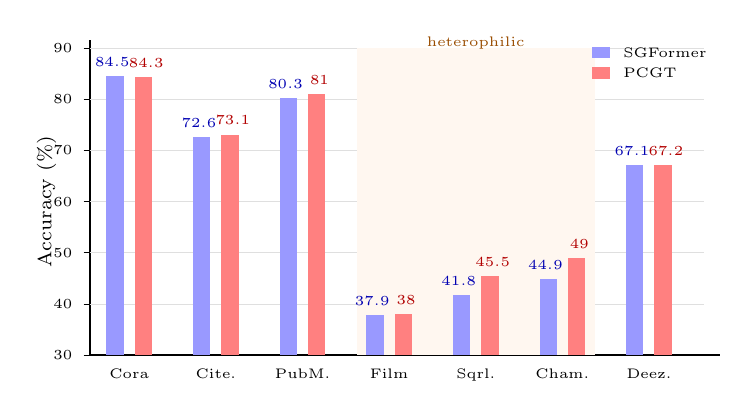
\begin{tikzpicture}[
  every node/.style={font=\scriptsize},
]
\pgfmathsetmacro{\bw}{0.22}  % bar width in cm
\pgfmathsetmacro{\gap}{0.14} % gap between paired bars
\pgfmathsetmacro{\sp}{1.1}   % spacing between groups

% Data: SGFormer and PCGT accuracies
% Cora 84.5/84.3, CiteSeer 72.6/73.1, PubMed 80.3/81.0, Film 37.9/38.0, Squirrel 41.8/45.5, Cham 44.9/49.0, Deezer 67.1/67.2

% Y-axis: show from 30 to 90, scale factor
\pgfmathsetmacro{\ymin}{30}
\pgfmathsetmacro{\yscale}{0.065}

% Draw axes
\draw[thick] (0,0) -- (0,{(90-\ymin)*\yscale+0.1});
\draw[thick] (0,0) -- ({7*\sp+0.3},0);

% Y-axis ticks and labels
\foreach \y/\lab in {30/30, 40/40, 50/50, 60/60, 70/70, 80/80, 90/90} {
  \draw (-0.08,{(\y-\ymin)*\yscale}) -- (0,{(\y-\ymin)*\yscale});
  \node[left, font=\tiny] at (-0.1,{(\y-\ymin)*\yscale}) {\lab};
}
% Y-axis label
\node[rotate=90, font=\scriptsize] at (-0.55,{(60-\ymin)*\yscale}) {Accuracy (\%)};

% Gridlines
\foreach \y in {40,50,60,70,80,90} {
  \draw[gray!25, thin] (0,{(\y-\ymin)*\yscale}) -- ({7*\sp+0.1},{(\y-\ymin)*\yscale});
}

% Heterophilic background zone (behind bars, subtle)
\fill[orange!6] ({3*\sp+0.5-\bw-\gap/2-0.12},0) rectangle ({5*\sp+0.5+\bw+\gap/2+0.12},{(90-\ymin)*\yscale});
\node[font=\tiny, orange!60!black] at ({4*\sp+0.5},{(91-\ymin)*\yscale}) {heterophilic};

% Bar data: {index}{label}{sgf_val}{pcgt_val}
\foreach \i/\lab/\sgf/\pcgt in {
  0/Cora/84.5/84.3,
  1/Cite./72.6/73.1,
  2/PubM./80.3/81.0,
  3/Film/37.9/38.0,
  4/Sqrl./41.8/45.5,
  5/Cham./44.9/49.0,
  6/Deez./67.1/67.2%
} {
  \pgfmathsetmacro{\xc}{\i*\sp+0.5}
  % SGFormer bar (blue)
  \fill[blue!40] ({\xc-\bw-\gap/2},0) rectangle ({\xc-\gap/2},{(\sgf-\ymin)*\yscale});
  % PCGT bar (red/orange)
  \fill[red!50] ({\xc+\gap/2},0) rectangle ({\xc+\bw+\gap/2},{(\pcgt-\ymin)*\yscale});
  % Value labels — offset left/right to avoid overlap
  \node[above, font=\tiny, blue!70!black, xshift=-1pt] at ({\xc-\bw/2-\gap/2},{(\sgf-\ymin)*\yscale}) {\pgfmathprintnumber[fixed, precision=1]{\sgf}};
  \node[above, font=\tiny, red!70!black, xshift=1pt] at ({\xc+\bw/2+\gap/2},{(\pcgt-\ymin)*\yscale}) {\pgfmathprintnumber[fixed, precision=1]{\pcgt}};
  % X-axis label
  \node[below, font=\tiny] at ({\xc},-0.05) {\lab};
}

% Legend
\fill[blue!40] ({5.8*\sp},  {(88-\ymin)*\yscale}) rectangle +(\bw,0.15);
\node[right, font=\tiny] at ({5.8*\sp+\bw+0.05},{(88-\ymin)*\yscale+0.075}) {SGFormer};
\fill[red!50]  ({5.8*\sp},  {(84-\ymin)*\yscale}) rectangle +(\bw,0.15);
\node[right, font=\tiny] at ({5.8*\sp+\bw+0.05},{(84-\ymin)*\yscale+0.075}) {PCGT};

\end{tikzpicture}
}% end resizebox
\caption{PCGT vs.\ SGFormer accuracy across all 7 datasets. PCGT shows the largest gains on heterophilic benchmarks (shaded), particularly Chameleon (+4.1\%) and Squirrel (+3.7\%).}
\label{fig:comparison}
\end{figure}

\subsection{Learned Parameters}

Analysis of the learned $\alpha$ and $\beta$ values reveals adaptive behavior:
\begin{itemize}
\item $\alpha$ (local vs.~global blend) stabilizes near 0.5 across datasets, indicating that both local and global attention contribute roughly equally with the current single-layer design.
\item $\beta$ (self-connection) is dataset-dependent and \emph{unconstrained}. On 9 of 11 datasets $\beta > 0$ (the model amplifies self-features), with the largest values on Squirrel ($\beta = +3.53$) and Chameleon ($\beta = +3.08$)---datasets with high-dimensional features (2089 and 2325 dims) where self-identity is highly informative. On Film ($\beta = -0.99 \pm 1.43$, negative in 8/10 splits) and Deezer ($\beta = -0.57 \pm 0.25$, negative in 5/5 runs), the model suppresses self-features. Notably, there is no linear correlation between $\beta$ and homophily (Pearson $r = 0.006$, $p = 0.99$ across all 11 datasets), suggesting that $\beta$ may reflect complementarity between self-features and attention-weighted context rather than homophily per se (though with only 11 datasets, this correlation test has limited statistical power).
\end{itemize}

\begin{figure}[t]
\centering
\resizebox{\columnwidth}{!}{%
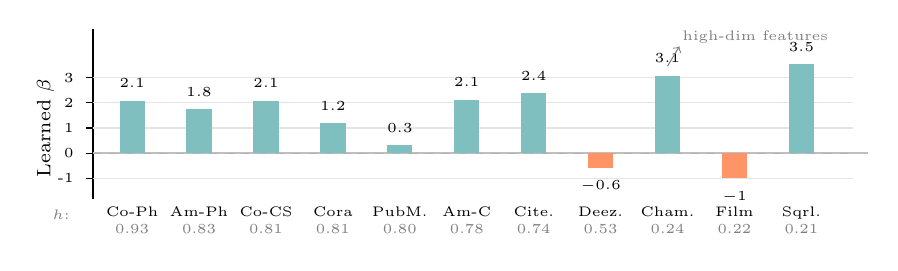
\begin{tikzpicture}[every node/.style={font=\scriptsize}]
\pgfmathsetmacro{\bw}{0.32}
\pgfmathsetmacro{\sp}{0.85}
\pgfmathsetmacro{\yscale}{0.32}

% Axes
\draw[thick] (0,-1.5*\yscale-0.1) -- (0,4.0*\yscale+0.3);
\draw[thick, gray!50] (0,0) -- ({11*\sp+0.5},0);

% Y ticks
\foreach \y in {-1,0,1,2,3} {
  \draw (-0.08,{\y*\yscale}) -- (0,{\y*\yscale});
  \node[left, font=\tiny] at (-0.12,{\y*\yscale}) {\y};
}
\node[rotate=90, font=\scriptsize] at (-0.6,{1.0*\yscale}) {Learned $\beta$};

% Gridlines
\foreach \y in {-1,1,2,3} {
  \draw[gray!20, thin] (0,{\y*\yscale}) -- ({11*\sp+0.3},{\y*\yscale});
}

% Zero line (dashed)
\draw[dashed, gray!60] (0,0) -- ({11*\sp+0.3},0);

% Data: all 11 datasets sorted by homophily (descending)
\foreach \i/\lab/\beta/\h in {
  0/Co-Ph/2.09/0.93,
  1/Am-Ph/1.75/0.83,
  2/Co-CS/2.08/0.81,
  3/Cora/1.19/0.81,
  4/PubM./0.31/0.80,
  5/Am-C/2.12/0.78,
  6/Cite./2.38/0.74,
  7/Deez./-0.57/0.53,
  8/Cham./3.08/0.24,
  9/Film/-0.99/0.22,
  10/Sqrl./3.53/0.21%
} {
  \pgfmathsetmacro{\xc}{\i*\sp+0.5}
  \pgfmathsetmacro{\bcolor}{\beta > 0 ? 1 : 0}
  \ifnum\bcolor=1
    \fill[teal!50] ({\xc-\bw/2},0) rectangle ({\xc+\bw/2},{\beta*\yscale});
    \node[above, font=\tiny] at ({\xc},{\beta*\yscale+0.04}) {\pgfmathprintnumber[fixed, precision=1]{\beta}};
  \else
    \fill[red!40!orange!60] ({\xc-\bw/2},0) rectangle ({\xc+\bw/2},{\beta*\yscale});
    \node[below, font=\tiny] at ({\xc},{\beta*\yscale-0.04}) {\pgfmathprintnumber[fixed, precision=1]{\beta}};
  \fi
  % X label — dataset name (horizontal) and homophily below
  \node[below, font=\tiny] at ({\xc},-1.5*\yscale-0.08) {\lab};
  \node[below, font=\tiny, gray] at ({\xc},-1.5*\yscale-0.3) {\h};
}

% Homophily row label
\node[font=\tiny, gray] at (-0.4,-1.5*\yscale-0.3) {$h$:};

% Annotation for Cham/Sqrl — placed above & to the right, no overlap
\draw[gray, thin, ->] ({8*\sp+0.5},{3.08*\yscale+0.12}) -- ++(0.15,0.25)
  node[above right, font=\tiny, inner sep=1pt] {high-dim features};

\end{tikzpicture}
}% end resizebox
\caption{Learned $\beta$ across all 11 datasets (sorted by homophily $h$, descending). Nine datasets learn $\beta > 0$; Film and Deezer learn $\beta < 0$. Chameleon/Squirrel learn the largest $\beta$ despite low $h$, likely due to high-dimensional features (2325/2089\,dims). Pearson $r{=}0.006$ ($p{=}0.99$): no linear correlation with homophily.}
\label{fig:beta}
\end{figure}

\subsection{Ablation Results}
\label{sec:ablation_results}

Table~\ref{tab:ablation} reports the contribution of each PCGT component on three representative datasets: Cora ($h$=0.81, homophilic), Chameleon ($h$=0.24, heterophilic), and Squirrel ($h$=0.21, heterophilic). Only the ablated component changes; all other hyperparameters remain identical.

\begin{table}[t]
\centering
\small
\resizebox{0.85\columnwidth}{!}{
\begin{tabular}{l|ccc}
\toprule
\textbf{Variant} & \textbf{Cora} & \textbf{Cham.} & \textbf{Sqrl.} \\
\midrule
\textbf{Full PCGT} & \best{84.77}{\scriptsize$\pm$.51} & \best{49.06}{\scriptsize$\pm$2.97} & \best{45.28}{\scriptsize$\pm$2.08} \\
\midrule
w/o Global & \runup{84.47}{\scriptsize$\pm$.50} & \runup{48.84}{\scriptsize$\pm$3.00} & \runup{45.11}{\scriptsize$\pm$2.06} \\
w/o Local & 84.23{\scriptsize$\pm$.76} & 48.67{\scriptsize$\pm$3.44} & 44.39{\scriptsize$\pm$1.69} \\
w/o PSE & 84.30{\scriptsize$\pm$.20} & 48.51{\scriptsize$\pm$3.34} & 44.64{\scriptsize$\pm$1.91} \\
w/o GCN & 70.90{\scriptsize$\pm$1.37} & 42.24{\scriptsize$\pm$3.26} & 37.59{\scriptsize$\pm$1.38} \\
Random part. & 83.78{\scriptsize$\pm$1.02} & 48.80{\scriptsize$\pm$2.07} & 44.60{\scriptsize$\pm$1.80} \\
\midrule
Pure GCN & 84.13{\scriptsize$\pm$.95} & 46.87{\scriptsize$\pm$2.49} & 41.84{\scriptsize$\pm$1.24} \\
SGFormer & 83.87{\scriptsize$\pm$.61} & 48.34{\scriptsize$\pm$2.64} & 44.81{\scriptsize$\pm$2.17} \\
\bottomrule
\end{tabular}
}
\caption{Ablation study (top) and reference comparisons (bottom). Each row removes one component. ``Pure GCN'' = GCN backbone only; ``SGFormer'' = SGFormer attention with identical hyperparameters. Ablation uses 5 runs with a fixed hyperparameter set for controlled comparison; absolute values may differ slightly from Table~\ref{tab:main} (10 runs, per-dataset tuning).}
\label{tab:ablation}
\end{table}

\textbf{Hybrid design is essential.}~~Removing the GCN branch causes large drops ($-$13.9, $-$6.8, $-$7.7), while Pure GCN alone trails full PCGT by $-$0.6 (Cora), $-$2.2 (Chameleon), and $-$3.4 (Squirrel). Neither branch alone matches the combination. This hybrid recipe---local message passing plus global attention---follows GraphGPS~\citep{rampasek2022graphgps} and similar architectures; the contribution here is the partition-conditioned attention that replaces the single-resolution alternatives. The PCGT attention branch's contribution grows with heterophily: +0.6$\to$+2.2$\to$+3.4 as homophily decreases, suggesting that partition-conditioned attention specifically helps where standard GCN aggregation hurts.

\textbf{PCGT vs.\ SGFormer under controlled comparison.}~~Running SGFormer with identical hyperparameters, PCGT wins by +0.9 (Cora), +0.7 (Chameleon), and +0.5 (Squirrel). This controls for hyperparameter tuning and isolates the architectural difference: multi-resolution partition attention outperforms single-resolution kernel approximation.

\textbf{Local attention more important than global.}~~Removing global attention costs $-$0.17 to $-$0.30, while removing local attention costs $-$0.39 to $-$0.89. Intra-partition exact attention captures richer patterns than the compressed cross-partition representations, particularly on heterophilic graphs where local community structure is most informative.

\textbf{PSE aids heterophilic classification.}~~Partition structural encoding provides its largest benefit on heterophilic datasets ($-$0.55 Chameleon, $-$0.64 Squirrel) vs.\ $-$0.47 on homophilic Cora. Explicit partition membership signals help distinguish structurally similar nodes across different communities.

\textbf{Topology-aware partitioning matters selectively.}~~Replacing METIS with random partitions hurts Squirrel ($-$0.68) more than Chameleon ($-$0.26). Both datasets have low homophily (Squirrel $h$=0.21, Chameleon $h$=0.24), but Squirrel's stronger community structure means METIS preserves more useful information. Chameleon, with $h$ near random chance ($1/K_{\text{class}} = 0.2$), benefits less---consistent with Deezer ($h \approx 0.5$), where random partitioning works about as well.

\subsection{Sensitivity to Partition Count \texorpdfstring{$K$}{K}}

Table~\ref{tab:ksweep} varies the number of partitions $K$ on Chameleon and Squirrel.

\begin{table}[t]
\centering
\resizebox{0.75\columnwidth}{!}{
\begin{tabular}{c|cc}
\toprule
$K$ & \textbf{Cham.} & \textbf{Sqrl.} \\
\midrule
5  & 48.65{\scriptsize$\pm$3.43} & \runup{45.30}{\scriptsize$\pm$2.01} \\
10 & \runup{49.06}{\scriptsize$\pm$2.97} & 45.28{\scriptsize$\pm$2.08} \\
15 & 48.94{\scriptsize$\pm$2.98} & 45.23{\scriptsize$\pm$2.00} \\
20 & 48.67{\scriptsize$\pm$3.27} & \best{45.32}{\scriptsize$\pm$1.81} \\
30 & \best{49.32}{\scriptsize$\pm$2.54} & 45.04{\scriptsize$\pm$1.96} \\
\bottomrule
\end{tabular}
}
\caption{Effect of partition count $K$. Default $K$=10. Performance is stable across $K \in \{5, 30\}$.}
\label{tab:ksweep}
\end{table}

\noindent PCGT is robust to the choice of $K$: Chameleon varies by only 0.67 points across $K \in \{5, 30\}$, and Squirrel by 0.28 points. This is a practical advantage---no expensive $K$-tuning is required.

\subsection{Runtime Analysis}

Table~\ref{tab:runtime} reports per-epoch wall-clock time on an NVIDIA H100 80GB GPU. We compare GCN (local message passing only), SGFormer ($O(N)$ global attention), and PCGT ($O(N^2/K + NMK)$ partition-conditioned attention plus GCN).

\begin{table}[t]
\centering
\small
\setlength{\tabcolsep}{3pt}
\resizebox{\columnwidth}{!}{%
\begin{tabular}{l|r|r|rrr|r}
\toprule
\textbf{Dataset} & $N$ & $K$ & \textbf{GCN} & \textbf{SGF} & \textbf{PCGT} & \textbf{Ratio} \\
\midrule
Cora       &  2,708  & 10  & 3.5  & 5.5   & 15.9  & 2.9$\times$ \\
CiteSeer   &  3,327  & 20  & 3.7  & 5.4   & 26.8  & 5.0$\times$ \\
PubMed     & 19,717  & 50  & 3.6  & 5.4   & 61.1  & 11.2$\times$ \\
Chameleon  &    890  & 10  & 2.4  & 4.6   & 15.1  & 3.3$\times$ \\
Squirrel   &  2,223  & 10  & 3.3  & 8.0   & 16.9  & 2.1$\times$ \\
Film       &  7,600  & 5   & 3.9  & 5.9   & 10.2  & 1.7$\times$ \\
Deezer     & 28,281  & 20  & 7.6  & 14.3  & 34.1  & 2.4$\times$ \\
Co-CS      & 18,333  & 15  & 4.0  & 6.4   & 22.3  & 3.5$\times$ \\
Co-Phys    & 34,493  & 20  & 6.6  & 9.9   & 30.5  & 3.1$\times$ \\
Am-Comp    & 13,752  & 10  & 4.2  & 6.5   & 17.9  & 2.7$\times$ \\
Am-Photo   &  7,650  & 10  & 3.4  & 5.6   & 16.9  & 3.0$\times$ \\
\midrule
ogbn-arxiv & 169,343 & 256 & ---  & 56.8  & 430.2 & 7.6$\times$ \\
\bottomrule
\end{tabular}
}% end resizebox
\caption{Per-epoch training time (ms) on H100. Ratio = PCGT / SGFormer. For medium-scale graphs ($N < 35$K), the overhead is 1.7--5.0$\times$; the PubMed outlier (11.2$\times$) reflects its large $K$=50. On ogbn-arxiv the overhead is 7.6$\times$, though both models complete 500 epochs in under 4 minutes.}
\label{tab:runtime}
\end{table}

\noindent \textbf{Overhead is moderate and predictable.} Across 11 medium-scale datasets, PCGT's overhead over SGFormer ranges from 1.7$\times$ (Film, $K$=5) to 5.0$\times$ (CiteSeer, $K$=20), with a median of 3.0$\times$. The overhead correlates with $K$ and $N$: smaller $K$ yields less intra-partition attention cost (cf.\ Film at 1.7$\times$ vs.\ PubMed at 11.2$\times$ with $K$=50). The PubMed outlier is explained by its large $K$=50, which creates $N^2/K \approx 7.8$M attention operations. On ogbn-arxiv (169K nodes), PCGT takes 430\,ms/epoch vs.\ SGFormer's 57\,ms, but even at this scale a full 500-epoch run completes in $\sim$3.6 minutes---practical for real-world use.
